\subsection{MUSIC-algoritmi}
\cite{Schmidt1986MultipleEstimation} kehitti MUSIC-algoritmin, joka perustuu mittausdatan jakamiseen keskenään ortogonaalisiin signaali- ja kohina-aliavaruuksiin. Tämän jälkeen tarkistetaan potentiaalisen lähdepisteen topografian kuuluminen signaaliavaruuteen \citep{Mosher1999SourceMUSIC}. Tällä menetelmällä lähteet kuvataan sähköisinä dipoleina ja algoritmi vaatii päämalliin tehdyn suoran mallin (\textit{forward model}). Suorassa mallissa täytyy ottaa huomioon pään ja aivojen geometriat sekä päänahan, kallon ja aivojen johtavuudet. \citep{hansen2010meg}

Tässä työssä oletetaan dipolien olevan kiinnitettyjä tiettyyn paikkaan. Dipolit voivat olla joko kiinteästi suuntautuneita eli niiden suuntaus tiedetään etukäteen tai vapaasti suuntautuvia, jolloin niiden suuntausta ei tiedetä. MUSIC-algoritmit voidaan jakaa kiinteän tai vapaan orientaation algoritmeihin. Kiinteän orientaation MUSIC-algoritmia sanotaan myös skalaari-MUSIC:ksi (\textit{scalar MUSIC}) sekä vapaan orientaation vektori-MUSIC:ksi (\textit{vector MUSIC}). \citep{Makela2018TruncatedLocalization}

Olkoon pisteessä \textbf{p} dipoli, jolla on momentti $\mathbf{q} = s\eta$, jossa $s$ on amplitudi ja $\eta$ on suuntaus. Tätä dipolia voidaan merkitä \textbf{(p,q)}. Mittaussensorien saamaa lukemaa merkitään $\mathbf{l(p,q)}$, jota sanotaan dipolin topografiaksi. Dipolin amplitudi voidaan olettaa vakioksi joten lineaarisuuden vuoksi $\mathbf{l(p,q)} = \mathbf{l(p,s\eta)} = s\mathbf{l(p,\eta)}$.

Muodostetaan johtokenttämatriisi (\textit{lead field matrix}) pisteeseen \textbf{p}:

\begin{equation}
    \mathbf{L(p) = [l(p,e_x),l(p,e_y),l(p,e_z)]}
\end{equation}
Tällöin topografia saa muodon $\mathbf{l(p},\eta)=\mathbf{L(p})\mathbf{\eta}(\mathbf{p})$.

Olkoon mittauksista saatu data koottu matriisin $\mathbf{Y}\in \mathbb{R}^{m\times N}$, jossa \textit{m} on mittaussensorien määrä ja \textit{N} mittausten lukumäärä. Oletetaan dipolien lukumäärän olevan $n$. Tällöin matriisi $\mathbf{Y}$ voidaan kirjoittaa muodossa:

\begin{equation}
    \mathbf{Y=AS+\varepsilon},
\end{equation}
jossa $\mathbf{A}\in \mathbb{R}^{m\times n}$ on sekoitusmatriisi (\textit{mixing matrix}), $\mathbf{S}\in \mathbb{R}^{n\times N}$ ajankulkumatriisi (\textit{time-course matrix}) ja $\mathbf{\varepsilon}$ mittauskohinaa. Matriisi \textbf{S} sisältää dipolien amplitudit tiettyinä ajanhetkinä.

Sekoitusmatriisi \textbf{A} muodostetaan eri tavalla riippuen siitä, käytetäänkö skalaari- vai vektori-MUSIC -algoritmia. Skalaari-MUSIC:n tapauksessa $\mathbf{A = [l(p_1),...,l(p_n)]}$ ja vektori-MUSIC:n tapauksessa $\mathbf{A = [L(p_1),...,L(p_n)]}$.

Data-avaruus $\text{span}(\mathbf{Y})$ jaetaan singulaariarvohajotelman avulla kahteen keskenään ortogonaaliseen aliavaruuteen, signaali-avaruuteen $\text{span}(\mathbf{A})$  ja kohina-avaruuteen $\text{span}(\mathbf{A^\bot})$ \citep{Mosher1999SourceMUSIC}. Olkoon matriisin \textbf{Y} singulaariarvohajotelma muotoa $\mathbf{Y = UDV}^T$ ja lähteiden määrä \textit{n}. Matriisin \textbf{D} diagonaalilla olevat \textit{n} ensimmäistä singulaariarvoa kuvaavat signaalia ja loput singulaariarvot kohinaa. Jos kohinaa $\varepsilon$ ei ole ja $\mathbf{A}$ oletetaan täysirankkiseksi, vektorit $\mathbf{U}(:,1:n)$ virittävät signaaliavaruuden eli $\text{span}(\mathbf{A}) = \mathbf{U}(:,1:n)$. Loput singulaarivektorit virittävät kohina-avaruuden. \citep{Mosher1999SourceMUSIC, Makela2018TruncatedLocalization} Ortogonaaliprojektio signaaliavaruuteen $\text{span}(\mathbf{A})$ voidaan ilmaista kaavan (\ref{eq:projektio}) avulla:

\begin{equation}
    \mathbf{P}_{sg}=\mathbf{U}(:,1:n)\mathbf{U}(:,1:n)^T
\end{equation} \citep{Makela2018TruncatedLocalization}

Lähteiden määrää ei aina tiedetä, joten se täytyy approksimoida. Todellisissa mittauksissa on myös aina kohinaa. Datamatriisin singulaariarvoista voidaan päätellä, kuinka monta voimakasta lähdettä löydetään signaaliavaruudesta. Singulaariarvoista voidaan muodostaa pylväsdiagrammi ja lähteiden määrä voidaan approksimoida sen mukaan, missä kohdassa tapahtuu merkittävä pudotus. Toisin sanoen suuret singulaariarvot kuvaavat lähteitä. Valkoisen kohinan tapauksessa pylväät tasoittuvat loppupäässä, kun lähteet ovat loppuneet. Värillisellä kohinalla pudotuksen löytäminen on hankalampaa ja täten lähteiden approksimaatio on vaikeampaa. Kuvassa \ref{fig:D} on simuloidun mittausdatan singulaariarvot pylväsdiagrammeina valkoisen ja värillisen kohinan tapauksissa.

\begin{figure}[h]
    \begin{minipage}{0.5\textwidth}
        \centering
        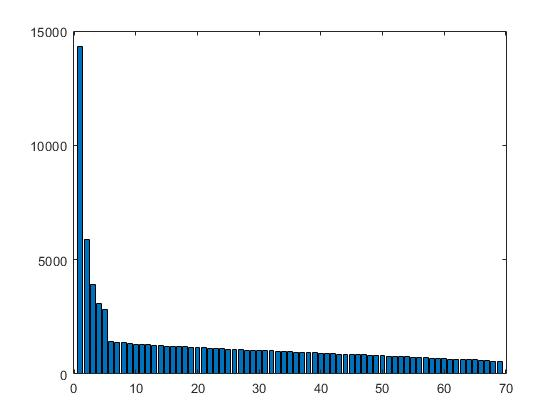
\includegraphics[width=\textwidth]{d_valk.jpg} 
    \end{minipage}
    \begin{minipage}{0.5\textwidth}
        \centering
        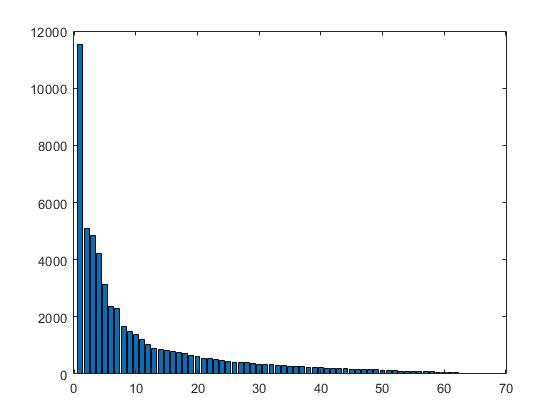
\includegraphics[width=\textwidth]{d_var.jpg}
    \end{minipage}
    \caption{Vasemman puoleisessa kuvassa simuloitu data sisältää valkoista kohinaa ja oikean puoleisessa kuvassa värillistä kohinaa. Molemmissa simulaatioissa on viisi lähdettä ja kohinan määrä on yhtä suuri.}
    \label{fig:D}
\end{figure}


Olkoon approksimoitujen lähteiden määrä \~n. Projektio voidaan nyt muodostaa approksimoitujen lähteiden määrän mukaan $\mathbf{P}_{s}=\mathbf{U}(:,1:\~n)\mathbf{U}(:,1:\~n)^T$, jolloin \~n jälkeiset singulaarivektorit kuvaavat kohinaa.

Pisteen $\mathbf{p}$ kuuluminen signaaliavaruuteen tarkistetaan projektio-operaattorin avulla. Pisteen $\mathbf{p}$ topografia $\mathbf{l(p)}$ lasketaan päämallin avulla. Topografia kuuluu signaaliavaruuteen, jos sen projektio signaaliavaruuteen on topografia itse. Toisin sanoen piste $\mathbf{p}$ on lähde, jos $\mathbf{P}_s\mathbf{l(p)} = \mathbf{l(p)}$. Jos $\mathbf{l(p)}$ sijaitsee signaaliavaruudessa, sen normi ei muutu projektiossa eli $||\mathbf{P}_s\mathbf{l(p)}||=||\mathbf{l(p)}||$. Jos $\mathbf{l(p)}$ ei sijaitse signaaliavaruudessa, sen projektion normi on pienempi kuin $\mathbf{l(p)}$:n normi eli
$||\mathbf{P}_s\mathbf{l(p)}||<||\mathbf{l(p)}||$. \citep{Makela2018TruncatedLocalization}

Näistä saadaan muodostettua paikannusfunktio (\textit{localizer function}) \citep{Makela2018TruncatedLocalization}, joka laskee jokaisen pisteen $\mathbf{p}$ kuulumisen signaaliavaruuteen

\begin{equation}
    \mathbf{\mu(p)} = \frac{||\mathbf{P}_s\mathbf{l(p)}||^2}{||\mathbf{l(p)}||^2} 
    \begin{cases}
    =1\text{, jos p on lähde}\\
    <1\text{, jos p ei ole lähde}
     \end{cases}
\end{equation}

Vapaan orientaation tapauksessa jokaiselle pisteelle $\mathbf{p}$ määräytyy suuntaus $\mathbf{\eta}$ mittausdatan perusteella. Vapaan orientaation MUSIC-algoritmia kutsutaan myös nimellä vektori-MUSIC (\textit{vector MUSIC}) \citep{Makela2018TruncatedLocalization}. Vektori-MUSIC muodostetaan hyvin samalla tavalla kuin skalaari-MUSIC, mutta sen paikannusfunktio on erilainen:

\begin{equation}
    \mathbf{\mu(p)} = \max_{||\eta||=1} \frac{||\mathbf{P}_s\mathbf{L(p)\eta}||^2}{||\mathbf{L(p)\eta}||^2}
\end{equation}

Vektori-MUSIC voidaan laskea ominaisarvojen avulla MATLAB:n avulla, joka esitetään liitteessä.